\chapter{Results and discussion}
\label{Final results}

\section{Composite objective function}
Two disciplines namely aerodynamics and structures which involves the calculation of aerodynamic drag ($ C_{DV} $) and von-Mises ($ \sigma _{v} $) stress are considered for shape optimization of airship profile. The aim is to have lowest possible aerodynamic drag and von-Mises stress. To achieve this, we need a composite objective function minimizing which, both $ C_{DV} $ and $ \sigma _{v} $ are minimized simultaneously. The composite objective function can be written as
\begin{equation}
F_{comp} = \frac{1}{2}\bigg( \frac{C_{DV}}{C_{DV,ref}} + \dfrac{\sigma _{v}}{\sigma _{v,ref}} \bigg)
\end{equation}

Where, $C_{DV,ref} , \sigma _{v,ref}  $ are the values of these parameters corresponding to the reference shape. This section presents the key results obtained in this study for the following three cases:
\begin{enumerate}
\item Axi-symmetric shape with minimum $ C_{DV}$ 
\item Non axi-symmetric shapes with minimum $ C_{DV}$
\item Non axi-symmetric shape with minimum $ \sigma_{v}$ 
\item Non axi-symmetric shape with minimum $ F_{comp}$ 

\end{enumerate}

\section{Axi-symmetric shape with minimum $ C_{DV}$}
Table \ref{optimal solution obtained} shows the design parameters of the optimal shape with minimum aerodynamic drag. It can be observed that the $ scale_y $ parameter is 1 which means the optimal shape is axi-symmetric. The results is obvious as given a fixed volume, axi-symmetric bodies will have minimum frontal area which is responsible for pressure drag. The shape is shown in Fig. \ref{Optimal min cdv case 1}

\begin{table}[H]
	\centering
	\caption{Parameters of axi-symmetric shape with minimum $ C_{DV}$}
	\label{optimal solution obtained}
	%\begin{ruledtabular}
	\begin{tabular}{ll}
		\hline \hline
		Design Parameters & Optimal value for minimum $ C_{DV} $    \\ \hline \hline
		
		$ Point\ of\ Max.\ Dia., m$ & 0.40910      \\  
		$ Nose\ Radius, r _{o} $ & 0.8    \\
		$ Tail\ Radius, r _{1} $ & 0.30428     \\  
		$ Prismatic\ Coeff., C _{p }$ & 0.61521 \\
		$ Fineness\ Ratio, \frac{l}{d} $ &5.69420 \\
		$Scaling\ in\ Y\ direction,\ scale\_y$ & 1 \\
		\hline \hline
		
		$ Kriging\ C_{DV} $ & 0.01796 \\
		$ von-Mises\ stress\ \sigma _{v}\ (Pa) $ & 403.47 \\ \hline \hline
	\end{tabular}
	%	\end{ruledtabular}
\end{table}

\begin{figure}[H]
	\centering
	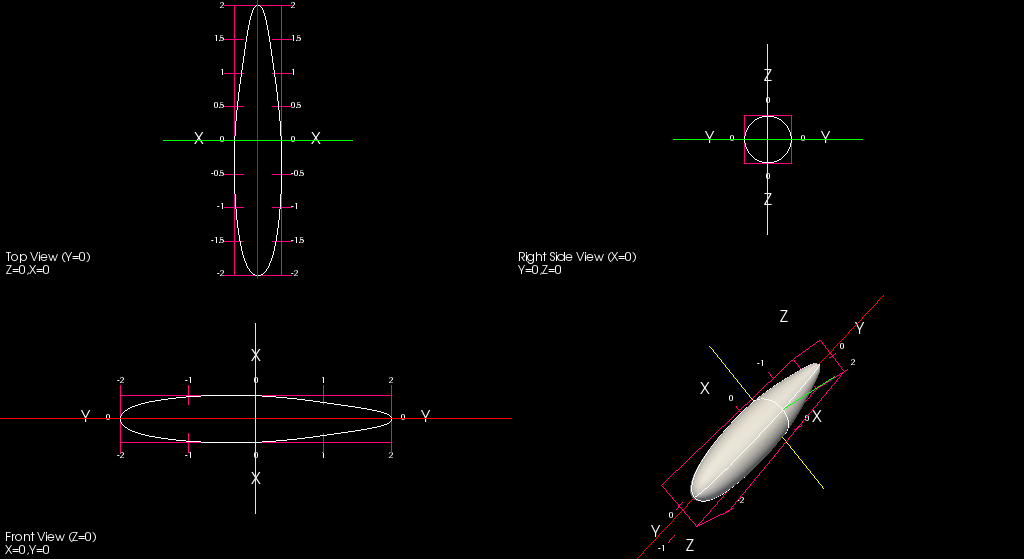
\includegraphics[width=450 pt]{rnd/min_cdv_case1.png}
	\caption{Axi-symmetric shape with minimum $ C_{DV}$}
	\label{Optimal min cdv case 1} %      only if needed
\end{figure}


\section{Non axi-symmetric shapes with minimum $ C_{DV}$}
\subsection*{Case A}
To obtain optimal shapes for non-axisymmetric shapes, the lower limits of $ Scale_y $ in genetic algorithm is changed from 1 to 2 i.e we are deceasing the size of design space and forcing the optimizer not to reach an axisymmetric shape. This is particularly useful when we have constraint on the curvature of envelope. The parameters of optimal shape obtained are shown in Table \ref{Optimal non-axisymmetric body obtained for mimimum Cdv case 2}. This shows that the drag has increased by 17.15 \%. The shape is shown in Fig.\ref{Optimal C DV non axi case 2}

\begin{table}[H]
	\centering
	\caption{Parameters of non axi-symmetric shapes with minimum $ C_{DV}$}
	\label{Optimal non-axisymmetric body obtained for mimimum Cdv case 2}
	%\begin{ruledtabular}
	\begin{tabular}{lc}
		\hline \hline
		Design Parameters & Optimal value for minimum $ C_{DV} $    \\ \hline \hline
		$ Point\ of\ Max.\ Dia., m$ & 0.37201      \\  
		$ Nose\ Radius, r _{o} $ & 0.62891    \\
		$ Tail\ Radius, r _{1} $ & 0.15214     \\  
		$ Prismatic\ Coeff., C _{p }$ & 0.64283 \\
		$ Fineness\ Ratio, \frac{l}{d} $ &5.53748 \\
		$Scaling\ in\ Y\ direction,\ scale\_y$ & 2.00000 \\ \hline \hline
		
		
		$ Kriging\ C_{DV} $ & 0.02064 \\
		$ von-Mises\ stress\  \sigma _{v} \ (Pa) $ & 415.29 \\
		
		\hline \hline
	\end{tabular}
	%	\end{ruledtabular}
\end{table}

\begin{figure}[H]
	\centering
	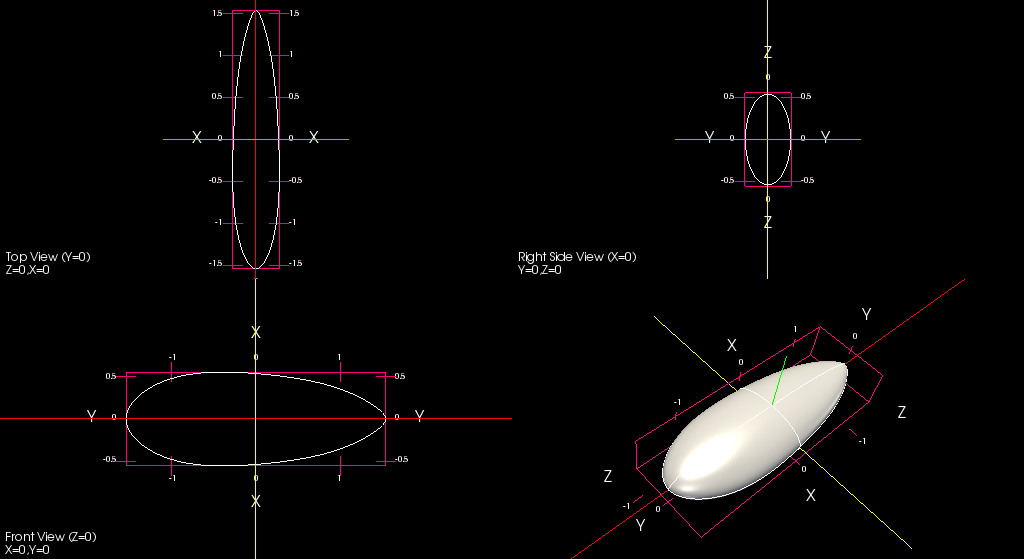
\includegraphics[width=450 pt]{rnd/min_cdv_case2.png}
	\caption{Non axi-symmetric shapes with minimum $ C_{DV}$}
	\label{Optimal C DV non axi case 2} %      only if needed
\end{figure}
\subsection*{Case B}
If we further change the lower limits of the genetic algorithm optimizer from 2 to 2.5, we obtain the following shape shown in Fig. \ref{Optimal min cdv} with parameters shown in Table \ref{Optimal non-axisymmetric body obtained for mimimum Cdv}.

\begin{table}[H]
	\centering
	\caption{Optimal non-axisymmetric envelope obtained for minimum $ C_{DV} $ case 3}
	\label{Optimal non-axisymmetric body obtained for mimimum Cdv}
	%\begin{ruledtabular}
	\begin{tabular}{lc}
		\hline \hline
		Design Parameters & Optimal value for minimum $ C_{DV} $    \\ \hline \hline
		$ Point\ of\ Max.\ Dia., m$ & 0.47998      \\  
		$ Nose\ Radius, r _{o} $ & 0.74580    \\
		$ Tail\ Radius, r _{1} $ & 0.17931     \\  
		$ Prismatic\ Coeff., C _{p }$ & 0.66849 \\
		$ Fineness\ Ratio, \frac{l}{d} $ & 5.81668 \\
		$Scaling\ in\ Y\ direction,\ scale\_y$ & 2.58996 \\ \hline \hline
		
		
		$ Kriging\ C_{DV} $ & 0.02204 \\
		$ von-Mises\ stress\  \sigma _{v} \ (Pa) $ & 401.01 \\
		
		\hline \hline
	\end{tabular}
	%	\end{ruledtabular}
\end{table}

\begin{figure}[H]
	\centering
	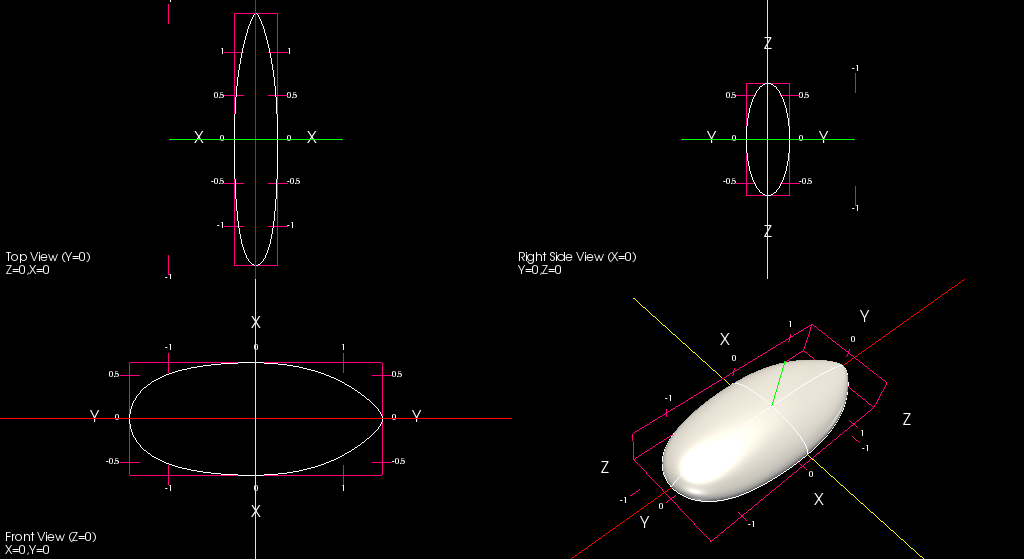
\includegraphics[width=450 pt]{rnd/min_cdv_case3.png}
	\caption{Non Axi-symmetric shapes with minimum $ C_{DV}$}
	\label{Optimal min cdv} %      only if needed
\end{figure}

\section{Non axi-symmetric shape with minimum $ \sigma_{v}$}

The parameters obtained and envelope shape for non axi-symmetric shape with minimum $ \sigma_{v}$ are shown in Table \ref{min_hoop_table} and Fig. \ref{min_hoop_fig} respectively.

\begin{table}[H]
	\centering
	%\begin{ruledtabular}
	\caption{Parameters of non Axi-symmetric shape with minimum $ \sigma_{v}$}
	\label{min_hoop_table}
	\begin{tabular}{lc}
		\hline \hline
		Design Parameters & Optimal value for minimum $ C_{DV} $    \\ \hline \hline
		$ Point\ of\ Max.\ Dia., m$ & 0.5      \\  
		$ Nose\ Radius, r _{o} $ & 0.8    \\
		$ Tail\ Radius, r _{1} $ & 0.5     \\  
		$ Prismatic\ Coeff., C _{p }$ & 0.55 \\
		$ Fineness\ Ratio, \frac{l}{d} $ &6 \\
		$Scaling\ in\ Y\ direction,\ scale\_y$ & 3 \\ \hline \hline
		
		
		$ Kriging\ C_{DV} $ & 0.02833
		 \\
		$ von-Mises\ stress\  \sigma _{v} \ (Pa) $ & 383.44 \\
		
		\hline \hline
	\end{tabular}
	%	\end{ruledtabular}
\end{table}

\begin{figure}[H]
	\centering
	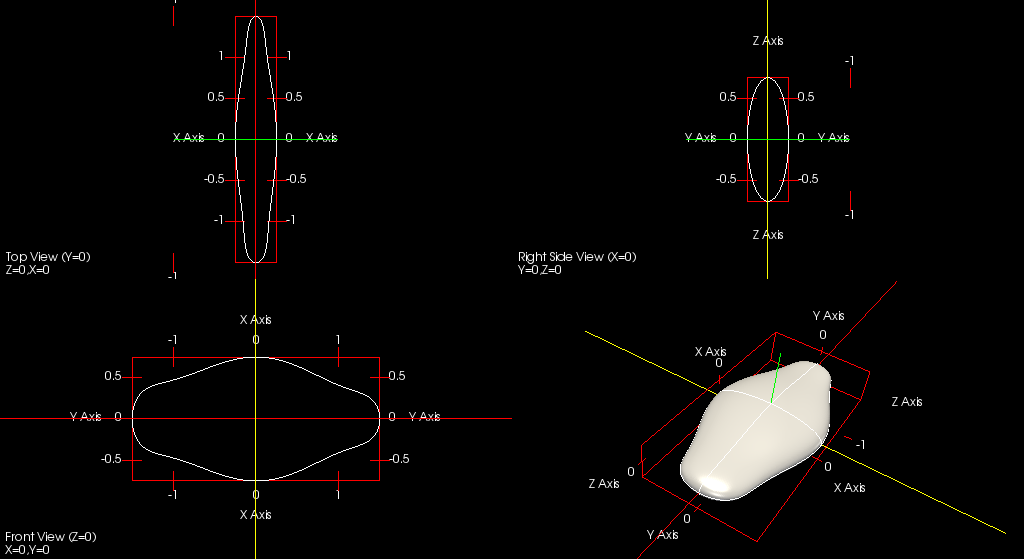
\includegraphics[width=450 pt]{rnd/min_von_mises.png}
	\caption{Non Axi-symmetric shape with minimum $ \sigma_{v}$}
	\label{min_hoop_fig}
\end{figure}

\section{Non axi-symmetric shape with minimum $ F_{comp}$}

The values of $C_{DV}$ and $ {\sigma _{v}} $ from Table \ref{Optimal non-axisymmetric body obtained for mimimum Cdv case 2} are taken as reference values for $C_{DV,ref}$ and $ {\sigma _{v,ref}} $ respectively. The composite objective function now becomes:
\begin{equation}
\label{eqn f comp}
F_{comp} = 0.5*(48.44* C_{DV} + 2.407e-3 * \sigma _{v})
\end{equation}

Since the bodies with $C_{DV} \ge 0.04 $ are not considered while developing the surrogate model, it cannot predict shapes with $C_{DV} \ge 0.04 $ with much confidence. So, $ F_{comp} $ has been modified with penalty function i.e when the optimizer is considering a shape with $C_{DV} \ge 0.04 $, we give huge penalty so that it wont go beyond 0.04. the Table \ref{Optimal non-axisymmetric body obtained for mimimum F comp} shows the optimal results obtained by minimizing Eqn. \ref{eqn f comp} using genetic algorithm. The parameters of shape obtained are shown in Table \ref{Optimal non-axisymmetric body obtained for mimimum F comp}.


\begin{table}[H]
	\centering
	\caption{parameters of non Axi-symmetric shape with minimum $ F_{comp}$}
	\label{Optimal non-axisymmetric body obtained for mimimum F comp}
	%\begin{ruledtabular}
	\begin{tabular}{lc}
		\hline \hline
		Design Parameters & Optimal value for minimum $ F_{comp} $    \\ \hline \hline

		$ Point\ of\ Max.\ Dia., m$ & 0.37207      \\  
		$ Nose\ Radius, r _{o} $ & 0.62949    \\
		$ Tail\ Radius, r _{1} $ & 0.15479    \\  
		$ Prismatic\ Coeff., C _{p }$ & 0.64237 \\
		$ Fineness\ Ratio, \frac{l}{d} $ & 5.63750 \\
		$Scaling\ in\ Y\ direction,\ scale\_y$ & 2.00000 \\ \hline \hline
		
		$ Kriging\ C_{DV} $ & 0.02069 \\
		$ von-Mises\ stress\  \sigma _{v} \ (Pa) $ & 413.52 \\
		$ F_{comp}$ & 0.99900 \\
		\hline \hline
	\end{tabular}
	%	\end{ruledtabular}
\end{table}


\begin{figure}[H]
	\centering
	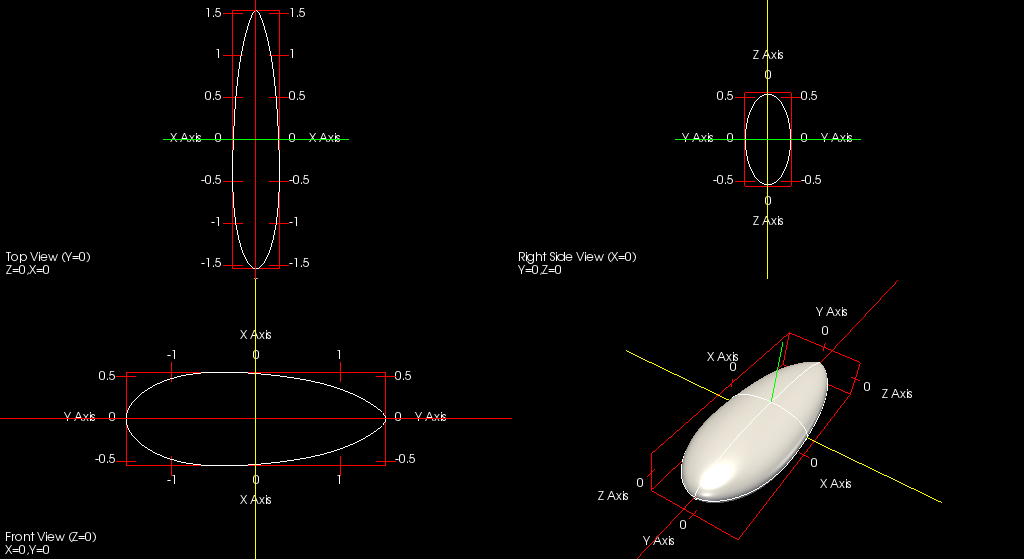
\includegraphics[width=450 pt]{rnd/min_F_comp.png}
	\caption{Non Axi-symmetric shape with minimum $ F_{comp}$}
\end{figure}



\chapter{Conclusions, Limitations and Future Work}
In the present study, a methodology for optimization of non-axisymmetric shapes has been developed. The same methodology can be used for the optimization of non-axisymmetric shaped submarines, hybrid airships and stratospheric airships with solar panels installed on the top side. 
The methodology parameterizes the envelope geometry, creates the geometrical shape and solves for drag using surrogate model. This surrogate model can be coupled as an alternate to CFD to find zero lift drag without having the need to run CFD every time in optimization routine. This helps the designer to find better shapes  using non-axisymmetric envelopes as he/she has more design space for exploration compared to axisymmetric shapes.
\section{Observations \& Conclusions} 
OpenFOAM software with its meshing, solving and post-processing capabilities are very helpful in performing 3D CFD analysis. The automatic mesh generation utility is found to be very helpful in automating the processes of optimization. 

The envelope geometry parameterization algorithm has found to be very efficient in capturing all the standard axisymmetric shapes [\citenum{alam2017thesis}] available in literature along with non-axisymmetric shapes given by Ceruti et al.[\citenum{Ceruti2013b}]



Kriging based surrogate models are found to be better in predicting the functional behaviour of numerical experiments. Kriging is even better than state of the art machine learning models. However the average accuracy is 3 \% with maximum percentage error being 6\%. This can be further improved by considering more number of points in Design Of Experiments (DOE) study. But because of time constraints, the 3\% accurate model has been coupled with optimizer. 

It has been observed that axisymmetric shapes are better for drag reduction however forcing the shape to be non-axisymmetric, the drag has been increased by 14.92 \%. This is particularly advantages when the percentage increase in other performance parameters like solar irradiation is very high for compromise of 14.92 \% increase in drag.

\section{Limitations of the present study}
The present study is limited to do only steady state CFD simulations for non-separating flows. However to study the effect of flow separation on bluff bodies like airships, unsteady CFD analysis has to be carried out. More accurate method is to consider aeroelastic effects on the drag. Moreover all the numbers for drag in present study are within 3\%.

\section{Future work}
It would be interesting to know the percentage increase in solar irradiation when the envelope gets flatter upper surface. The trade off between solar irradiation and drag can be studied. The envelope geometry parameterization can further be modified to capture cambered and multi lobe bodies which is very useful for hybrid airships and submarines. 
